%% This file is a portion of the source for Revised Edition 1.1 of
%% Operating Systems and Middleware: Supporting Controlled
%% Interaction, Copyright 2011 by Max Hailperin.  This work is
%% licensed under the Creative Commons Attribution-ShareAlike 3.0
%% Unported License. To view a copy of this license, visit
%% http://creativecommons.org/licenses/by-sa/3.0/ or send a letter to
%% Creative Commons, 171 Second Street, Suite 300, San Francisco,
%% California, 94105, USA.
\chapter{Threads}
\label{threads-chapter}
\section{Introduction}
Computer programs consist of instructions, and computers carry out
sequences of computational steps specified by those instructions.  We
call each sequence of computational steps that are strung together one after
another a \vocab{thread}.  The simplest programs to write are
single-threaded, with instructions that should be executed one after
another in a single sequence.  However, in
Section~\ref{threads-example-section}, you will learn how to write
programs that produce more than one thread of execution, each an
independent sequence of computational steps, with few if any
ordering constraints between the steps in one thread and those in
another.  Multiple threads can also come into existence by running
multiple programs, or by running the same program more than once.

Note the distinction between a program and a thread; the program
contains instructions, whereas the thread consists of the execution of
those instructions.  Even for single-threaded programs, this
distinction matters.  If a program contains a loop, then a very short
program could give rise to a very long thread of execution.  Also,
running the same program ten times will give rise to ten threads, all
executing one program.  Figure~\ref{scan-2-1} summarizes how threads
arise from programs.
\begin{figure}
\centerline{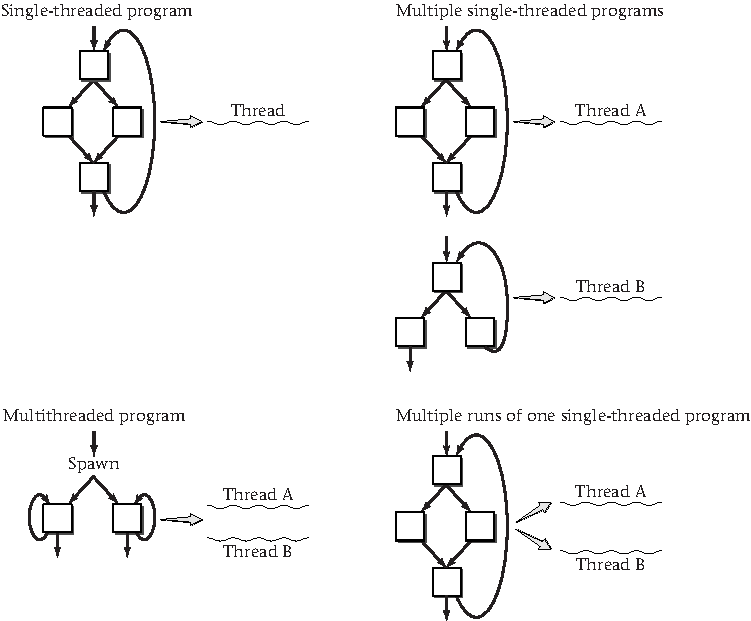
\includegraphics{hail_f0201}}
\caption{Programs give rise to threads.}
\label{scan-2-1}
\end{figure}

Each thread has a lifetime, extending from the time its first
instruction execution occurs until the time of its last instruction
execution.  If two threads have overlapping lifetimes, as illustrated
in Figure~\ref{scan-2-2}, we say they are
\vocab{concurrent}.
\begin{figure}
\centerline{\includegraphics{hail_f0202}}
\caption{Sequential and concurrent threads}
\label{scan-2-2}
\end{figure}
One of the most fundamental goals of an operating system is to allow
multiple threads to run concurrently on the same computer.  That is,
rather than waiting until the first thread has completed before a
second thread can run, it should be possible to divide the computer's
attention between them.  If the computer hardware includes multiple
processors, then it will naturally be possible to run threads
concurrently, one per processor.  However, the operating system's
users will often want to run more concurrent threads than the hardware
has processors, for reasons described in Section~\ref{threads-uses-section}.  Therefore, the operating
system will need to divide each processor's attention between multiple
threads.  In this introductory textbook I will mostly limit myself
to the case of all the threads needing to be run on a
single processor.  I will explicitly indicate those places where I
do address the more general multi-processor case.

In order to make the concept of concurrent threads concrete,
Section~\ref{threads-example-section} shows how to write a program
that spawns multiple threads each time the program is run.  Once you
know how to create threads, I will explain in
Section~\ref{threads-uses-section} some of the reasons why it is
desirable to run multiple threads concurrently and will offer some
typical examples of the uses to which threads are put.

These first two sections explain the application programmer's view of
threads: how and why the programmer would use concurrent threads.
This sets us up for the next question: how does the operating system
support the application programmer's desire for concurrently executing
threads?  In Sections \ref{threads-switching-section} and
\ref{threads-preemptive-section}, we will examine how the system does
so.  In this chapter, we will consider only the fundamentals of how
the processor's attention is switched from one thread to another.  Some
of the related issues I address in other chapters include deciding
which thread to run at each point (Chapter~\ref{scheduling-chapter})
and controlling interaction among the threads (Chapters
\ref{synchronization-chapter}, \ref{transactions-chapter},
\ref{vm-chapter}, and \ref{processes-chapter}).
Also, as explained in Chapter~\ref{intro-chapter}, I will wait until
Chapter~\ref{processes-chapter} to explain the protection boundary
surrounding the operating system.  Thus, I will need to wait until
that chapter to distinguish threads that reside entirely within that
boundary, threads provided from inside the boundary for use outside of
it, and threads residing entirely outside the boundary (known as
\foldvocabs{user-level}{thread} or, in Microsoft Windows, \vocabs{fiber}).

Finally, the chapter concludes with the standard features of this
book: a brief discussion of security issues, followed by exercises,
programming and exploration projects, and notes.

\section{Example of Multithreaded Programs}\label{threads-example-section}

Whenever a program initially starts running, the computer carries
out the program's instructions in a single thread. Therefore, if the program is intended
to run in multiple threads, the original thread needs at some point to
spawn off a child thread that does some actions, while the parent
thread continues to do others.  (For more than two threads, the
program can repeat the thread-creation step.)  Most programming
languages have an application programming interface (or API) for
threads that includes a way to create a child thread.  In this
section, I will use
the Java API and the API for C that is called \vocabs{pthread}, for
\vocabs{POSIX thread}.  (As you will see throughout the book, POSIX is a
comprehensive specification for UNIX-like systems, including many APIs
beyond just thread creation.)

Realistic multithreaded programming requires the control of thread
interactions, using techniques I show in
Chapter~\ref{synchronization-chapter}.  Therefore, my examples in
this chapter are quite simple, just enough to show the spawning of
threads.

To demonstrate the independence of the two threads, I will have both
the parent and the child thread respond to a timer.  One will sleep
three seconds and then print out a message.  The other will sleep five
seconds and then print out a message.  Because the threads execute
concurrently, the second message will appear approximately two seconds
after the first.  (In Programming Projects
\ref{first-threads-program-input-time},
\ref{second-threads-program-input-time}, and \ref{third-threads-program-input-time},
you can write a somewhat
more realistic program, where one thread responds to user input and
the other to the timer.)

Figure~\ref{Simple2Threads} shows the Java version of this program.
The \verb|main| program first creates a
\index{Thread class@\verb"|Thread"| class}\verb|Thread| object called
\verb|childThread|.  The
\index{Runnable interface@\verb"|Runnable"| interface}\verb|Runnable| object associated
with the child thread has a \verb|run| method that sleeps three
seconds (expressed as 3000
milliseconds) and then prints a message.  This \verb|run| method starts
running when the main procedure invokes \verb|childThread.start()|.
Because the \verb|run| method is in a separate thread, the main thread
can continue on to the subsequent steps, sleeping five seconds (5000 milliseconds)
and printing its own message.
\begin{figure}
\begin{verbatim}
public class Simple2Threads {
  public static void main(String args[]){
    Thread childThread = new Thread(new Runnable(){
        public void run(){
          sleep(3000);
          System.out.println("Child is done sleeping 3 seconds.");
        }
      });
    childThread.start();
    sleep(5000);
    System.out.println("Parent is done sleeping 5 seconds.");
  }

  private static void sleep(int milliseconds){
    try{
      Thread.sleep(milliseconds);
    } catch(InterruptedException e){
      // ignore this exception; it won't happen anyhow
    }
  }
}
\end{verbatim}
\caption{A simple multithreaded program in Java}
\label{Simple2Threads}
\end{figure}

Figure~\ref{simple2threads} is the equivalent program in C, using the
pthreads API.  The \verb|child| procedure sleeps three seconds and prints a
message.  The \verb|main| procedure creates a \verb|child_thread|
running the \verb|child| procedure, and then itself sleeps
five seconds and prints a message.  The most significant difference from the
Java API is that
\index{pthread_create@\verb"|pthread_create"|}\verb|pthread_create|
both creates the child thread and starts it running, whereas in Java
those are two separate steps.
\begin{figure}
\begin{verbatim}
#include <pthread.h>
#include <unistd.h>
#include <stdio.h>

static void *child(void *ignored){
  sleep(3);
  printf("Child is done sleeping 3 seconds.\n");
  return NULL;
}

int main(int argc, char *argv[]){
  pthread_t child_thread;
  int code;

  code = pthread_create(&child_thread, NULL, child, NULL);
  if(code){
    fprintf(stderr, "pthread_create failed with code %d\n", code);
  }
  sleep(5);
  printf("Parent is done sleeping 5 seconds.\n");
  return 0;
}
\end{verbatim}
\caption{A simple multithreaded program in C}
\label{simple2threads}
\end{figure}

In addition to portable APIs, such as the Java and pthreads APIs, many
systems provide their own non-portable APIs.  For example, Microsoft
Windows has the Win32 API, with procedures such as \index{CreateThread@\verb"|CreateThread"|}\verb|CreateThread|
and \index{Sleep@\verb"|Sleep"|}\verb|Sleep|.  In Programming Project~\ref{win32-threads-program}, you can modify the
program from Figure~\ref{simple2threads} to use this API.

\section{Reasons for Using Concurrent Threads}\label{threads-uses-section}
You have now seen how a single execution of one program can result in
more than one thread.  Presumably, you were already at least somewhat
familiar with generating multiple threads by running multiple
programs, or by running the same program multiple times.  Regardless
of how the threads come into being, we are faced with a question.  Why
is it desirable for the computer to execute multiple threads
concurrently, rather than waiting for one to finish before starting
another?
Fundamentally, most uses for concurrent threads serve one of two goals:
\begin{description}
\item[Responsiveness:] allowing the computer system to respond quickly
  to something external to the system, such as a human user or another
  computer system.  Even if one thread is in the midst of a long
  computation, another thread can respond to the external agent.  Our
  example programs in Section~\ref{threads-example-section}
  illustrated responsiveness: both the parent and the child thread
  responded to a timer.
\item[Resource utilization:] keeping most of the hardware resources
  busy most of the time.  If one thread has no need for a
  particular piece of hardware, another may be able to make productive
  use of it.
\end{description}
Each of these two general themes has many variations, some of which we
explore in the remainder of this section.  A third reason why
programmers sometimes use concurrent threads is as a tool for
modularization.  With this, a complex system may be decomposed into a group of
interacting threads.

Let's start by considering the responsiveness of a web server, which provides many client
computers with the specific web pages they request over the Internet.
Whenever a client computer makes a network connection to the server,
it sends a sequence of bytes that contain the name of the desired web
page.  Therefore, before the server program can respond, it needs to
read in those bytes, typically using a loop that continues reading in
bytes from the network connection until it sees the end of the
request.  Suppose one of the clients is connecting using a very slow
network connection, perhaps via a dial-up modem.  The server may read
the first part of the request and then have to wait a considerable
length of time before the rest of the request arrives over the network.  What
happens to other clients in the meantime?  It would be
unacceptable for a whole website to grind to a halt, unable to serve
any clients, just waiting for one slow client to finish issuing its
request.  One way some web servers avoid this unacceptable situation
is by using multiple threads, one for each client connection, so that
even if one thread is waiting for data from one client, other threads
can continue interacting with the other clients.
Figure~\ref{scan-2-3} illustrates the unacceptable single-threaded web
server and the more realistic multithreaded one.
\begin{figure}
\centerline{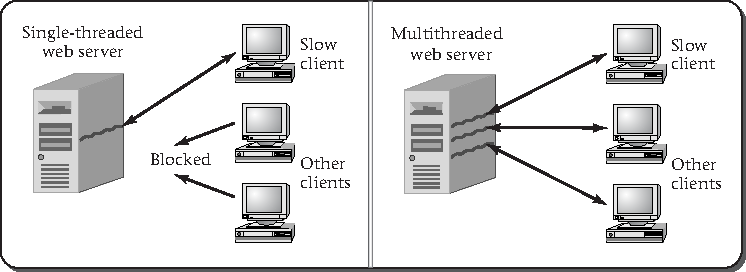
\includegraphics{hail_f0205}}
\caption{Single-threaded and multithreaded web servers}
\label{scan-2-3}
\end{figure}

On the client side, a web browser may also illustrate the need for
responsiveness.  Suppose you start loading in a very large web page,
which takes considerable time to download.  Would you be happy
if the computer froze up until the download finished?
Probably not.  You expect to be able to work on a spreadsheet in a
different window, or scroll through the first part of the web page to
read as much as has already downloaded, or at least click on the
Stop button to give up on the time-consuming download.  Each of
these can be handled by having one thread tied up loading the web page
over the network, while another thread is responsive to your actions
at the keyboard and mouse.

This web browser scenario also lets me foreshadow later portions of
the textbook concerning the controlled interaction between threads.
Note that I sketched several different things you might want
to do while the web page downloaded.  In the first case, when you work
on a spreadsheet, the two concurrent threads have almost nothing to do
with one another, and the operating system's job, beyond allowing them
to run concurrently, will mostly consist of isolating each from the
other, so that a bug in the web browser doesn't overwrite part of your
spreadsheet, for example.  This is generally done by encapsulating the
threads in separate protection environments known as \vocabes{process}, as we
will discuss in Chapters \ref{vm-chapter} and \ref{processes-chapter}.  (Some systems call processes
\vocabs{task}, while others use \vocab{task} as a synonym for \vocab{thread}.)
If, on the other hand, you continue using the browser's user interface
while the download continues, the concurrent threads are closely
related parts of a single application, and the operating system need
not isolate the threads from one another.  However, it may still need
to provide mechanisms for regulating their interaction.  For example,
some coordination between the downloading thread and the
user-interface thread is needed to ensure that you can scroll through
as much of the page as has been downloaded, but no further.  This
coordination between threads is known as \vocab{synchronization} and is
the topic of Chapters \ref{synchronization-chapter} and \ref{transactions-chapter}.

Turning to the utilization of hardware resources, the most obvious
scenario is when you have a dual-processor computer.  In this case, if
the system ran only one thread at a time, only half the processing
capacity would ever be used.  Even if the human user of the computer
system doesn't have more than one task to carry out, there may be
useful housekeeping work to keep the second processor busy.  For
example, most operating systems, if asked to allocate memory for an
application program's use, will store all zeros into the memory first.
Rather than holding up each memory allocation while the zeroing is
done, the operating system can have a thread that proactively zeros
out unused memory, so that when needed, it will be all ready.  If this
housekeeping work (zeroing of memory) were done on demand, it would
slow down the system's real work; by using a concurrent thread to
utilize the available hardware more fully, the performance is
improved.  This example also illustrates that not all threads need to
come from user programs.  A thread can be part of the operating system
itself, as in the example of the thread zeroing out unused memory.

Even in a single-processor system, resource utilization considerations
may justify using concurrent threads.  Remember that a computer
system contains hardware resources, such as
disk drives, other than the processor. Suppose you have two tasks to complete on your PC: you
want to scan all the files on disk for viruses, and you want to do a
complicated photo-realistic rendering of a three-dimensional scene
including not only solid objects, but also shadows cast on
partially transparent smoke clouds.  From experience, you know
that each of these will take about an hour.  If you do one and then
the other, it will take two hours.  If instead you do the two
concurrently---running the virus scanner in one window while you run
the graphics rendering program in another window---you may be
pleasantly surprised to find both jobs done in only an hour and a half.

The explanation for the half-hour savings in elapsed time is that the virus scanning program spends most
of its time using the disk drive to read files, with only modest
bursts of processor activity each time the disk completes a read
request, whereas the rendering program spends most of its time doing
processing, with very little disk activity.  As illustrated in Figure~\ref{scan-2-4}, running them in
sequence leaves one part of the computer's hardware idle much of the time,
whereas running the two concurrently keeps the processor and disk
drive both busy, improving the overall system efficiency.
\begin{figure}
\centerline{\includegraphics{hail_f0206}}
\caption{Overlapping processor-intensive and disk-intensive activities}
\label{scan-2-4}
\end{figure}
Of course,
this assumes the operating system's scheduler is smart enough to let
the virus scanner have the processor's attention (briefly) whenever a
disk request completes, rather than making it wait for the rendering
program.  I will address this issue in Chapter~\ref{scheduling-chapter}.

As you have now seen, threads can come from multiple sources and serve
multiple roles.  They can be internal portions of the operating
system, as in the example of zeroing out memory, or part of the user's
application software.  In the latter case, they can either be dividing
up the work within a multithreaded process, such as the web server
and web browser examples, or can come from multiple independent
processes, as when a web browser runs in one window and a spreadsheet
in another.  Regardless of these variations, the typical reasons
for running the threads concurrently remain unchanged: either to provide
increased responsiveness or to improve system efficiency by more fully
utilizing the hardware.  Moreover, the basic mechanism used to divide
the processor's attention among multiple threads remains the same in
these different cases as well; I describe that mechanism in Sections
\ref{threads-switching-section} and \ref{threads-preemptive-section}.
Of course, some cases require the additional protection mechanisms
provided by processes,
which we discuss in Chapters \ref{vm-chapter} and
\ref{processes-chapter}.  However, even then, it is still necessary to
leave off work on one thread and pick up work on another.

\section{Switching Between Threads}\label{threads-switching-section}

In order for the operating system to have more than one thread
underway on a processor, the system needs to have some mechanism for
switching attention between threads.  In particular, there needs to be
some way to leave off from in the middle of a thread's sequence of
instructions, work for a while on other threads, and then pick back up
in the original thread right where it left off.  In order to explain
\foldindex{thread}{switching}thread switching as simply as possible, I will initially assume that
each thread is executing code that contains, every once in a while,
explicit instructions to temporarily switch to another thread.  Once
you understand this mechanism, I can then build on it for the more
realistic case where the thread contains no explicit thread-switching
points, but rather is automatically interrupted for thread switches.

Suppose we have two threads, A and B, and we use A1, A2, A3, and so forth as
names for the instruction execution steps that constitute A, and
similarly for B.  In this case, one possible execution sequence might
be as shown in Figure~\ref{scan-2-5}.  As I will explain subsequently,
when thread A executes \verb|switchFromTo(A,B)| the computer starts
executing instructions from thread B.
\begin{figure}
\centerline{\begin{tabular}{ll}
\multicolumn{1}{c}{\textbf{Thread A}}&\multicolumn{1}{c}{\textbf{Thread B}}\\
A1&\\
A2&\\
A3&\\
\texttt{switchFromTo(A,B)}&\\
&B1\\
&B2\\
&B3\\
&\texttt{switchFromTo(B,A)}\\
A4&\\
A5&\\
\texttt{switchFromTo(A,B)}&\\
&B4\\
&B5\\
&B6\\
&B7\\
&\texttt{switchFromTo(B,A)}\\
A6&\\
A7&\\
A8&\\
\texttt{switchFromTo(A,B)}&\\
&B8\\
&B9
\end{tabular}}
\caption{Switching between threads}
\label{scan-2-5}
\end{figure}
In a more realistic example, there might be more than two threads, and
each might run for many more steps (both between switches and overall), with
only occasionally a new thread starting or an existing thread exiting.

Our goal is that the steps of each thread form a coherent execution
sequence.  That is, from the perspective of thread A, its execution
should not be much different from one in which A1 through A8 occurred
consecutively, without interruption, and similarly for thread B's
steps B1 through B9.  Suppose, for example, steps A1 and A2 load two
values from memory into registers, A3 adds them, placing the sum in a
register, and A4 doubles that register's contents, so as to get twice
the sum.  In this case, we want to make sure that A4 really does
double the sum computed by A1 through A3, rather than doubling some
other value that thread B's steps B1 through B3 happen to store in the same
register.  Thus, we can see that switching threads cannot simply be a
matter of a jump instruction transferring control to the appropriate
instruction in the other thread.  At a minimum, we will also have to
save registers into memory and restore them from there, so that when a
thread resumes execution, its own values will be back in the
registers.

In order to focus on the essentials, let's put aside the issue of how
threads start and exit.  Instead, let's focus just on the normal case where one
thread in progress puts itself on hold and switches to another thread
where that other thread last left off, such as the switch from A5 to
B4 in the preceding example.  To support switching threads,
the operating system will need to keep information about each thread,
such as at what point that thread should resume execution. If this
information is stored in a block of memory for each thread, then we
can use the addresses of those memory areas to refer to the threads.
The block of memory containing information about a thread is
called a \foldvocab{thread}{control block} or
\foldvocab{task}{control block} (\vocab{TCB}).  Thus, another way of
saying that we use the addresses of these blocks is to say that we use
pointers to thread control blocks to refer to threads.

Our fundamental thread-switching mechanism will be the
\verb|switchFromTo| procedure, which takes two of these
thread control block pointers as parameters: one specifying the
thread that is being switched out of, and one specifying the next
thread, which is being switched into.  In our running example,
\verb|A| and \verb|B| are pointer variables pointing to
the two threads' control blocks, which we use alternately in the
roles of outgoing thread and next thread.  For example, the program for
thread A contains code after instruction A5 to switch from
\verb|A| to \verb|B|, and the program for thread B
contains code after instruction B3 to switch from
\verb|B| to \verb|A|. Of course, this assumes that each
thread knows both its own identity and the identity of the thread to
switch to.  Later, we will see how this unrealistic assumption can be
eliminated.  For now, though, let's see how we could write the
\verb|switchFromTo| procedure so that
\verb|switchFromTo(A, B)| would save the current execution
status information into the structure pointed to by \verb|A|,
read back previously saved information from the structure pointed to
by \verb|B|, and resume where thread B left off.

We already saw that the execution status information to save includes
not only a position in the program, often called the \vocab{program counter}
(\vocab{PC}) or \vocab{instruction pointer} (\vocab{IP}), but also the contents of registers.
Another critical part of the execution status for programs compiled
with most higher level language compilers is a portion of the memory
used to store a stack, along with a stack pointer register that
indicates the position in memory of the current top of the stack.  You
likely have encountered this form of storage in some prior
course---computer organization, programming language principles, or
even introduction to computer science.  If not,
Appendix~\ref{stacks-appendix} provides the information you will need
before proceeding with the remainder of this chapter.

When a thread resumes execution, it must find the stack
the way it left it.  For example, suppose thread A pushes two items on the
stack and then is put on hold for a while, during which thread B executes.
When thread A resumes execution, it should find the two items it pushed at
the top of the stack---even if thread B did some pushing of its own
and has not yet gotten around to popping.  We can arrange for this by
giving each thread its own stack, setting aside a separate portion of
memory for each of them.  When thread A is executing, the \vocab{stack
pointer} (or SP register) will be pointing somewhere within thread A's
stack area, indicating how much of that area is occupied at that time.
Upon switching to thread B, we need to save away A's stack pointer,
just like other registers, and load in thread B's stack pointer.  That
way, while thread B is executing, the stack pointer will move up and
down within B's stack area, in accordance with B's own pushes and
pops.

Having discovered this need to have separate stacks and switch stack
pointers, we can simplify the saving of all other registers by
pushing them onto the stack before switching and popping them off the
stack after switching, as shown in Figure~\ref{scan-2-6}.
\begin{figure}
\centerline{\includegraphics{hail_f0208}}
\caption{Saving registers in thread control blocks and per-thread stacks}
\label{scan-2-6}
\end{figure}
We can use this approach to outline the
code for switching from the outgoing thread to the next
thread, using \verb|outgoing| and \verb|next| as
the two pointers to thread control blocks.
(When switching from \verb|A| to \verb|B|, \verb|outgoing| will be
\verb|A| and \verb|next| will be \verb|B|.  Later, when switching back
from \verb|B| to \verb|A|, \verb|outgoing| will be \verb|B| and
\verb|next| will be \verb|A|.)
We will use
\verb|outgoing->SP| and \verb|outgoing->IP| to refer to two slots within the
structure pointed to by \verb|outgoing|, the slot used to save the stack
pointer and the one used to save the instruction pointer.  With these
assumptions, our code has the following general form:
\begin{verbatim}
  push each register on the (outgoing thread's) stack
  store the stack pointer into outgoing->SP
  load the stack pointer from next->SP
  store label L's address into outgoing->IP
  load in next->IP and jump to that address
L:
  pop each register from the (resumed outgoing thread's) stack
\end{verbatim}
Note that the code before the label (\verb|L|) is done at the time of
switching away from the outgoing thread, whereas the code after that
label is done later, upon resuming execution when some other thread
switches back to the original one.

This code not only stores the outgoing thread's stack pointer
away, but also restores the next thread's stack pointer.  Later, the
same code will be used to switch back.  Therefore, we can count on the
original thread's stack pointer to have been restored when control
jumps to label \verb|L|.  Thus, when the registers are popped, they
will be popped from the original thread's stack, matching the pushes
at the beginning of the code.

We can see how this general pattern plays out in a real system, by
looking at the thread-switching code from the Linux operating system
for the i386 architecture. (The i386 architecture is also known as the
x86 or IA-32; it is a popular processor architecture used in
standard personal computer processors such as Intel's Core, Xeon, and Atom
families and AMD's FX and Opteron families.)
If you don't want to see real code, you can skip ahead to
the paragraph after the block of assembly code.  However, even if you aren't familiar with i386 assembly language, you
ought to be able to see how this code matches the preceding pattern.

This
is real code extracted from the Linux kernel, though with some
peripheral complications left out.  The
stack pointer register is named \verb|%esp|, and when this code starts running, the
registers known as \verb|%ebx| and \verb|%esi| contain the \verb|outgoing|
and \verb|next| pointers, respectively.  Each of those pointers is the
address of a
thread control block. The location at offset 812 within the TCB contains
the thread's instruction pointer, and the location at offset 816 contains
the thread's stack pointer.  (That is, these memory locations contain
the instruction pointer and stack pointer to use when resuming that
thread's execution.)  The code surrounding the thread switch does not
keep any important values in most of the other registers; only the
special flags register and the register named \verb|%ebp| need to
be saved and restored.  With that as background, here is the
code, with explanatory comments:
%examplesource: linux-2.6.0-test1/include/asm-i386/system.h in linux-2.6.0-test1/kernel/sched.c
%exampleedit: the ret was really jmp __switch_to
\begin{verbatim}
   pushfl                 # pushes the flags on outgoing's stack
   pushl %ebp             # pushes %ebp on outgoing's stack
   movl %esp,816(%ebx)    # stores outgoing's stack pointer
   movl 816(%esi),%esp    # loads next's stack pointer
   movl $1f,812(%ebx)     # stores label 1's address,
                          #    where outgoing will resume
   pushl 812(%esi)        # pushes the instruction address
                          #    where next resumes
   ret                    # pops and jumps to that address
1: popl %ebp              # upon later resuming outgoing,
                          #    restores %ebp
   popfl                  # and restores the flags
\end{verbatim}

Having seen the core idea of how a processor is switched from running
one thread to running another, we can now eliminate the assumption
that each thread switch contains the explicit names of the outgoing
and next threads.  That is, we want to get away from having to name
threads \verb|A| and \verb|B| in
\verb|switchFromTo(A, B)|.  It is easy enough to know
which thread is being switched away from, if we just keep track at all
times of the currently running thread, for example, by storing a
pointer to its control block in a global variable called
\verb|current|.  That leaves the question of which thread is being
selected to run next.  What we will do is have the operating system
keep track of all the threads in some sort of data structure, such as
a list.  There will be a procedure, \verb|chooseNextThread()|, which
consults that data structure and, using some scheduling policy, decides
which thread to run next.  In Chapter~\ref{scheduling-chapter}, I will explain how
this scheduling is done; for now, take it as a black box.
Using this tool, one can write a procedure, \verb|yield()|, which
performs the following four steps:
\begin{verbatim}
outgoing = current;
next = chooseNextThread();
current = next;   // so the global variable will be right
switchFromTo(outgoing, next);
\end{verbatim}
Now, every
time a thread decides it wants to take a break and let other threads
run for a while, it can just invoke \verb|yield()|.
This is essentially the approach taken by real systems, such as Linux.
One complication in a \index{multiprocessor system}multiprocessor system is that the \verb|current|
thread needs to be recorded on a per-processor basis.

Thread switching is often called \foldvocab{context}{switching}, because it
switches from the execution context of one thread to that of another
thread.  Many authors, however, use the phrase \foldvocab{context}{switching} differently,
to refer to switching processes with their protection contexts---a
topic we will discuss in Chapter~\ref{processes-chapter}.  If the distinction matters,
the clearest choice is to avoid the ambiguous term
\foldvocab{context}{switching}
 and use the more specific \foldvocab{thread}{switching} or
\foldvocab{process}{switching}.

Thread switching is the most common form of
\vocab{dispatching} a thread, that is, of causing a processor to
execute it.  The only way a thread can be dispatched without a thread switch
is if a processor is idle.

\section{Preemptive Multitasking}\label{threads-preemptive-section}
At this point, I have explained thread switching well enough for
systems that employ \foldvocab{cooperative}{multitasking}, that is, where each
thread's program contains explicit code at each point where a thread
switch should occur.  However, more realistic operating systems use what
is called \foldvocab{preemptive}{multitasking}, in which the program's code
need not contain any thread switches, yet thread switches will none
the less automatically be performed from time to time.

One reason to prefer preemptive
multitasking is because it means that buggy code in one
thread cannot hold all others up.  Consider, for example, a loop that
is expected to iterate only a few times; it would seem safe, in a
cooperative multitasking system, to put thread switches only before
and after it, rather than also in the loop body.  However, a bug could
easily turn the loop into an infinite one, which would hog the
processor forever.  With preemptive multitasking, the thread may still
run forever, but at least from time to time it will be put on hold and
other threads allowed to progress.

Another reason to prefer preemptive multitasking is that it allows
thread switches to be performed when they best
achieve the goals of responsiveness and resource utilization.  For
example, the operating system can preempt a thread when input becomes
available for a waiting thread or when a hardware device falls idle.

Even with preemptive multitasking,
it may occasionally be useful for a thread to voluntarily give way to
the other threads, rather than to run as long as it is allowed.
Therefore, even preemptive systems normally provide
\verb|yield()|.
The name varies depending on the API, but often has \verb|yield| in it;
for example, the pthreads API uses the name \verb|sched_yield()|.  One
exception to this naming pattern is the Win32 API of Microsoft
Windows, which uses the name \verb|SwitchToThread()| for the equivalent
of \verb|yield()|.

Preemptive multitasking does not need any fundamentally different
thread switching mechanism; it simply needs the addition of a hardware
interrupt mechanism. In case you are not familiar with how interrupts
work, I will first take a moment to review this aspect of hardware
organization.

Normally a processor will execute consecutive instructions one after
another, deviating from sequential flow only when directed by an
explicit jump instruction or by some variant such as the \verb|ret|
instruction used in the Linux code for thread switching.
However, there is always some mechanism by which external hardware
(such as a disk drive or a network interface) can signal that it needs
attention.
A hardware timer can also be set to demand attention periodically,
such as every millisecond.
When an I/O device or timer needs attention, an \vocab{interrupt} occurs, which is almost as
though a procedure call instruction were forcibly inserted between the
currently executing instruction and the next one.  Thus, rather than
moving on to the program's next instruction, the processor jumps off
to the special procedure called the \vocab{interrupt
handler}.

The interrupt handler, which is part of the operating
system, deals with the hardware device and then executes a \vocab{return
from interrupt} instruction, which jumps back to the instruction that
had been about to execute when the interrupt occurred.  Of course, in
order for the program's execution to continue as expected, the
interrupt handler needs to be careful to save all the registers at the
start and restore them before returning.

Using this interrupt mechanism, an operating system can provide
preemptive multitasking.  When an interrupt occurs, the interrupt
handler first
saves the registers to the current thread's stack and
takes care of the immediate needs, such as
accepting data from a network interface controller or updating the
system's idea of the current time by one millisecond.  Then,
rather than simply restoring the registers and executing a return from
interrupt instruction, the interrupt handler checks whether it would
be a good time to preempt the current thread and switch to another.

For example, if the interrupt signaled the arrival of data for which a
thread had long been waiting, it might make sense to switch to
that thread.  Or, if the interrupt was from the timer and the current
thread had been executing for a long time, it may make sense to give
another thread a chance.  These policy decisions are related to
scheduling, the topic of Chapter~\ref{scheduling-chapter}.

In any case, if the
operating system decides to preempt the current thread, the interrupt
handler switches threads using a
mechanism such as the \verb|switchFromTo| procedure.
This switching of threads includes switching to the new thread's stack,
so when the interrupt handler restores registers before returning,
it will be restoring the new thread's registers. The previously running
thread's register values will remain safely on its own stack until that
thread is resumed.

\section{Security and Threads}

One premise of this book is that every topic raises its own security
issues.  Multithreading is no exception.  However, this section will
be quite brief, because with the material covered in this chapter, I can present only the
security problems connected with multithreading, not the
solutions.  So that I do not divide problems from their solutions, this
section provides only a thumbnail sketch, leaving serious
consideration of the problems and their solutions to the chapters that
introduce the necessary tools.

Security issues arise
when some threads are unable to execute because others are hogging the
computer's attention.  Security issues also arise because of unwanted
interactions between threads. Unwanted interactions include a thread writing into storage
that another thread is trying to use or reading from storage another
thread considers confidential.  These problems are most
likely to arise if the programmer has a difficult time understanding
how the threads may interact with one another.

The security section in Chapter~\ref{scheduling-chapter} addresses the
problem of some threads monopolizing the computer.  The security
sections in Chapters \ref{synchronization-chapter},
\ref{transactions-chapter}, and \ref{processes-chapter} address the
problem of controlling threads' interaction.  Each of these chapters
also has a strong emphasis on design approaches that make interactions
easy to understand, thereby minimizing the risks that arise from
incomplete understanding.

\section*{Exercises}
\begin{chapterEnumerate}
\item
Based on the examples in Section~\ref{threads-example-section},
name at least one difference between the \verb|sleep| procedure in the
POSIX API and the \verb|Thread.sleep| method in the Java API.
\item
Give at least three more examples, beyond those given in the text,
where it would be useful to run more concurrent threads on a computer
than that computer's number of processors.  Indicate how your examples
fit the general reasons to use concurrency listed in the text.
\item
Suppose thread A goes through a loop 100 times, each time performing
one disk I/O operation, taking 10~milliseconds, and then some computation, taking
1~millisecond.  While each 10-millisecond disk operation is in progress, thread A cannot
make any use of the processor.  Thread B runs for 1 second,
purely in the processor, with no I/O.  One millisecond
of processor time is spent each time the processor switches
threads; other than this switching cost, there is no problem with the
processor working on thread B during one of thread A's I/O operations.  (The
processor and disk drive do not contend for memory access bandwidth,
for example.)
\begin{enumerate}
\item
Suppose the processor and disk work purely on thread A until its
completion, and then the processor switches to thread B and runs all of
that thread.  What will the total elapsed time be?
\item
Suppose the processor starts out working on thread A, but every time
thread A performs a disk operation, the processor switches to B during
the operation and then back to A upon the disk operation's completion.
What will the total elapsed time be?
\end{enumerate}
\item
Consider a uniprocessor system where each arrival of input from an
external source triggers the creation and execution of a new thread,
which at its completion produces some output.  We are interested in
the response time from triggering input to resulting output.
\begin{enumerate}
\item
Input arrives at time 0 and again after 1~second, 2~seconds, and so forth.
Each arrival triggers a thread that takes 600~milliseconds to run.
Before the thread can run, it must be created and dispatched, which
takes 10~milliseconds.  What is the average response time for these
inputs?
\item
Now a second source of input is added, with input arriving at times
0.1~seconds, 1.1~seconds, 2.1~seconds, and so forth.  These inputs trigger
threads that only take 100~milliseconds to run, but they still need
10~milliseconds to create and dispatch.  When an input arrives, the
resulting new thread is not created or dispatched until the processor
is idle.  What is the average response time for this second class of
inputs?  What is the combined average response time for the two
classes?
\item
Suppose we change the way the second class of input is handled.  When
the input arrives, the new thread is immediately created and
dispatched, even if that preempts an already running thread.  When the
new thread completes, the preempted thread resumes execution after a
1~millisecond thread switching delay.  What is the average response
time for each class of inputs?  What is the combined average for the
two together?
\end{enumerate}
\item
When control switches away from a thread and later switches back to
that thread, the thread resumes execution where it left off.
Similarly, when a procedure calls a subroutine and later the
subroutine returns, execution picks back up where it left off in the
calling procedure.  Given this similarity, what is the essential
difference between thread switching and subroutine call/return?  You saw
that each thread has a separate stack, each in its own area of
memory.  Why is this not necessary for subroutine invocations?
\end{chapterEnumerate}

\section*{Programming Projects}
\begin{chapterEnumerate}
\item\label{first-threads-program-input-time}
If
you program in C, read the documentation for
\index{pthread_cancel@\verb"|pthread_cancel"|}\verb|pthread_cancel|.
Using this information and the model provided in
Figure~\ref{simple2threads} on page~\pageref{simple2threads},
write a program where the initial
(main) thread creates a second thread.  The main thread should
read input from the keyboard, waiting until the user presses the Enter key.  At that point, it should kill off the
second thread and print out a message reporting that it has done so.
Meanwhile, the second thread should be in an infinite loop, each time
around sleeping five seconds and then printing out a message.  Try
running your program.  Can the sleeping thread print its periodic
messages while the main thread is waiting for keyboard input?  Can the
main thread read input, kill the sleeping thread, and print a message
while the sleeping thread is in the early part of one of its
five-second sleeps?
\item\label{second-threads-program-input-time}
If you
program in Java, read the documentation for the
\verb|stop| method in the \verb|Thread|
class.  (Ignore the information about it being deprecated.  That will
make sense only after you read Chapter~\ref{synchronization-chapter} of
this book.)  Write the program described in Programming Project~\ref{first-threads-program-input-time},
except do so in Java.  You can use the program shown in
Figure~\ref{Simple2Threads} on page~\pageref{Simple2Threads} as a model.
\item\label{third-threads-program-input-time}
Read the API documentation for some programming language other than C,
C$++$, or Java to find out how to spawn off a thread and how to
sleep.  Write a program in this language equivalent to the Java and C
example programs in Figures \ref{Simple2Threads} and
\ref{simple2threads} on pages \pageref{Simple2Threads} and
\pageref{simple2threads}.  Then do the equivalent of Programming
Projects \ref{first-threads-program-input-time} and \ref{second-threads-program-input-time} using the language you have chosen.
\item\label{win32-threads-program}
If you program in C under Microsoft Windows, you can use the
native Win32 API instead of the portable pthreads API. Read the
documentation of \verb|CreateThread| and \verb|Sleep| and modify the
program of Figure~\ref{simple2threads} on
page~\pageref{simple2threads} to use these procedures.
\end{chapterEnumerate}

\section*{Exploration Projects}
\begin{chapterEnumerate}
\item
Try the experiment of running a disk-intensive process and a
processor-intensive process concurrently.  Write a report carefully
explaining what you did and in which hardware and software system context
you did it, so that someone else could replicate your
results.  Your report should show how the elapsed time for the
concurrent execution compared with the times from sequential
execution.  Be sure to do multiple trials and to reboot the system
before each run so as to eliminate effects that come from keeping disk
data in memory for re-use.  If you can find documentation for any
performance-monitoring tools on your system, which would provide
information such as the percentage of CPU time used or the number of
disk I/O operations per second, you can include this information in
your report as well.
\item
Early versions of Microsoft Windows and Mac~OS used cooperative
multitasking.  Use the web, or other sources of information, to find
out when each switched to preemptive multitasking.  Can you find and
summarize any examples of what was written about this change at the
time?
\item
How frequently does a system switch threads?  You can find this out on
a Linux system by using the \verb|vmstat| program.  Read the
man page for \verb|vmstat|, and then run it to find the number of context
switches per second.
Write a report in which you carefully
explain what you did and the hardware and software system context in
which you did it, so that someone else could replicate your
results.
\end{chapterEnumerate}

\section*{Notes}
The idea of executing multiple threads concurrently seems to have
occurred to several people (more or less concurrently) in the late
1950s.  They did not use the word \vocab{thread}, however.  For example, a
1959 article by \index{Codd, E. F.@Codd, E.~F.}E.~F.\ Codd et al.~\cite{max984} stated that
``the second form of parallelism, which we shall call {\em nonlocal},
provides for concurrent execution of instructions which need not be
neighbors in an instruction stream, but which may belong, if you
please, to entirely separate and unrelated programs.''  From the
beginning, authors were aware of both reasons for using concurrency that I have emphasized
(resource utilization and responsiveness).  The same article by Codd
et al., for example, reports that ``one object of concurrently
running tasks which belong to different (perhaps totally unrelated)
programs is to achieve a more balanced loading of the facilities than
would be possible if all the tasks belonged to a single program.
Another object is to achieve a specified real-time response in a
situation in which messages, transactions, etc., are to be processed
on-line.''

I mentioned that an operating system may dedicate a thread to
preemptively zeroing out memory.  One example of this is the \vocab{zero
page thread} in Microsoft Windows.  See
\index{Russinovich, Mark E.}Russinovich and \index{Solomon, David A.}Solomon's
book~\cite{max981} for details.

I extracted the Linux thread switching code from version 2.6.0-test1
of the kernel.  Details (such as the offsets 812 and 816) may differ
in other versions.  The kernel source code is written in a combination
of assembly language and C, contained in
\verb|include/asm-i386/system.h| as included into
\verb|kernel/sched.c|.  To obtain pure assembly code, I fed the
source through the \verb|gcc| compiler.  Also, the \verb|ret|
instruction is a simplification; the actual kernel at that point jumps
to a block of code that ends with the \verb|ret| instruction.

My brief descriptions of the \index{POSIX}POSIX and \index{Java API}Java APIs are intended only as
concrete illustrations of broader concepts, not as a replacement for
documentation of those APIs.  You can find the official documentation
on the web at \textit{\url{http://opengroup.org/unix}}
and \textit{\url{http://www.oracle.com/technetwork/java/index.html}},
respectively.
